\documentclass[aspectratio=169]{beamer}
\usepackage[english]{babel}
\usepackage[utf8]{inputenc}

% AMSLaTeX packages
\usepackage{amsthm}
\usepackage{amsmath}
\usepackage{amsfonts}
\usepackage[algoruled]{algorithm2e}

\usetheme{default}
\useoutertheme{default}
% we want to use images
\usepackage{graphicx}
\usepackage{movie15}
\usepackage{hyperref}

% table relates packages
\usepackage{booktabs}
\usepackage{multirow}
% pick a font
\usepackage{palatino}           
% \usepackage{times}
\usepackage{tikz}
\usetikzlibrary[positioning,arrows,decorations.pathmorphing,backgrounds,fit,calc]
% \AtBeginSection[]  % "Beamer, do the following at the start of every section"
% {
%   \begin{frame}<beamer> 
%     \frametitle{Outline} % make a frame titled "Outline"
%     \tableofcontents[currentsection]  % show TOC and highlight current section
%   \end{frame}                    
% }

% \AtBeginSubsection[]
% {
%   \begin{frame}
%     \frametitle{Outline}
%     \tableofcontents[currentsection,currentsubsection]
%   \end{frame}
% }

\AtBeginSection[]
{
   \begin{frame}
       \frametitle{Outline}
       \tableofcontents[currentsection]
   \end{frame}
}

\newcommand{\ebox}[1][1em]{\framebox[#1]{\phantom{M}}}

\setlength\arraycolsep{1.4pt}% some length

%gets rid of navigation symbols
\setbeamertemplate{navigation symbols}{}

%gets rid of bottom navigation bars
\setbeamertemplate{footline}[page number]{}
\setbeamertemplate{headline}{}


\usepackage{movie15}
\usebackgroundtemplate{
\includegraphics[width=\paperwidth]{../templates/NormalANLBlue}}
\title{An Introduction to Multiobjective Simulation Optimization\\with ParMOO}
\author{Tyler Chang}
\institute{Mathematics and Computer Science Division,\\
Argonne National Laboratory}
\date{\today}
\begin{document}

\setbeamertemplate{footline}{}
{
\usebackgroundtemplate{
\includegraphics[width=\paperwidth]{../templates/TitleANLBlue}}

\frame{\titlepage}
}

\setbeamertemplate{footline}[page number]{}

% FRAME: overview
%\begin{frame}
%  \frametitle{Outlines}
%  \tableofcontents
%\end{frame}
% ========================================
% main slides come here
% ========================================
\begin{frame}\frametitle{Review of Single-Objective Optimization}
\begin{columns}
\begin{column}{0.5\textwidth}
\begin{center}

\pause

\includegraphics[width=0.2\textwidth]{chip-icon.jpg}

\bigskip
\bigskip

\pause

\hrule

{\small place new component}

\end{center}
\end{column}
\begin{column}{0.5\textwidth}
\bigskip
{\Large

\pause
$$
\min_{x\in[0,1]} f(x)
$$

\pause
$$
f(x) = \text{dist}(x, \text{chip})^2
$$

\pause
$$
f(x) = x^2
$$
}
\end{column}
\end{columns}
\end{frame}

\begin{frame}\frametitle{Gradient Descent}
\begin{center}
\onslide<1>{
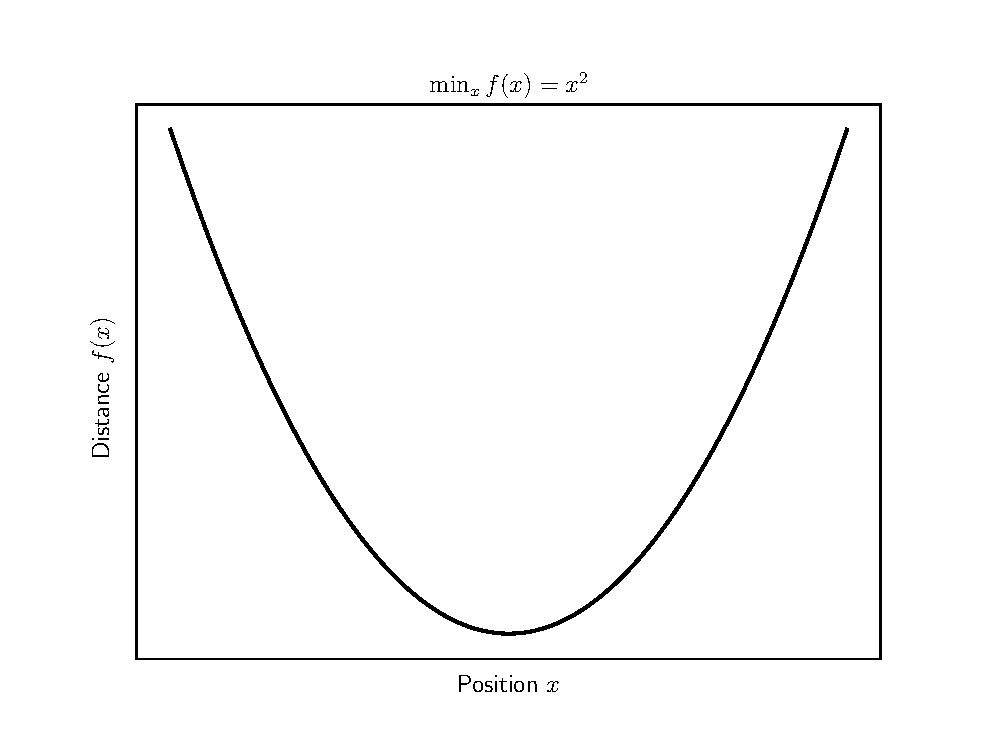
\includegraphics[height=2in]{single_obj_pt1.eps}
}

\vskip -2in

\onslide<2>{
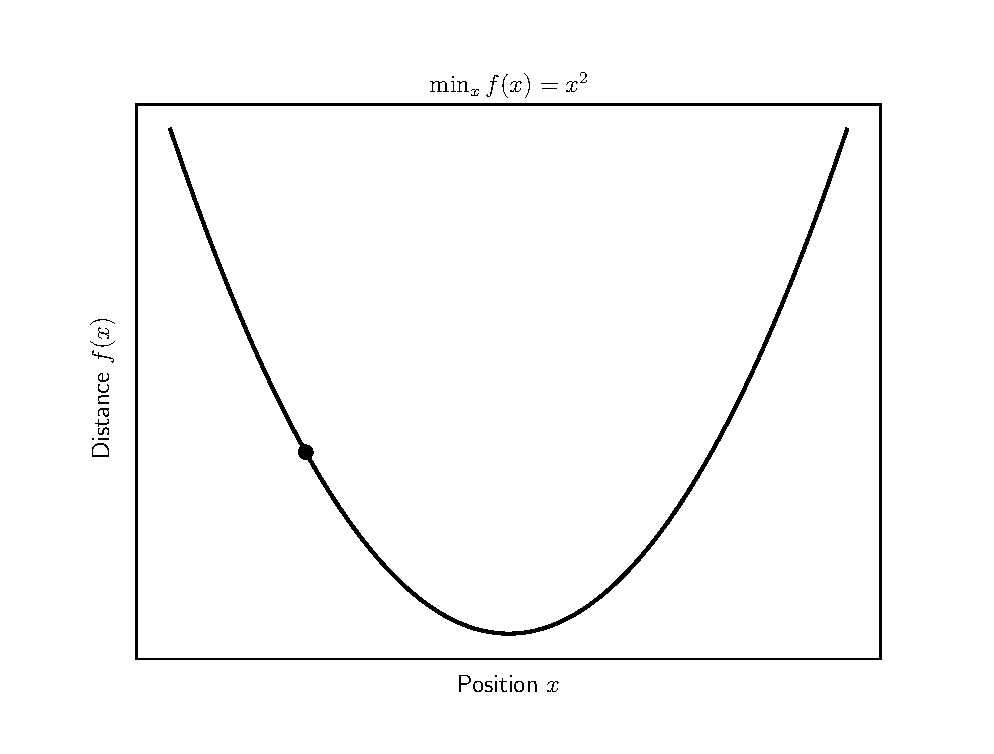
\includegraphics[height=2in]{single_obj_pt2.eps}
}

\vskip -2in

\onslide<3>{
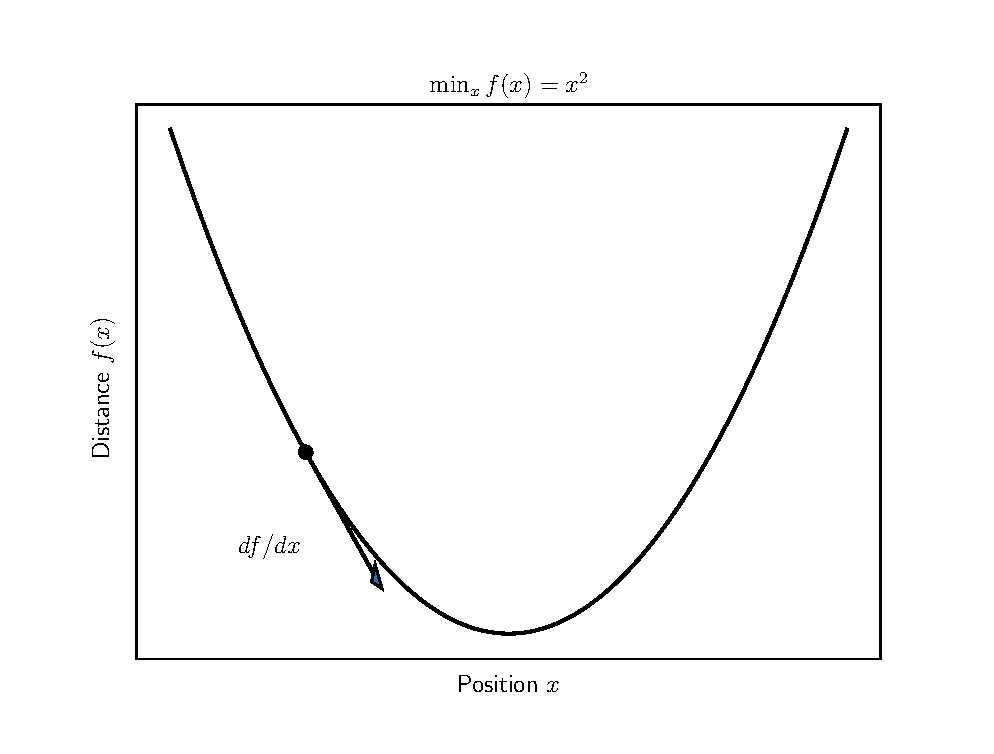
\includegraphics[height=2in]{single_obj_pt3.eps}
}
\end{center}
\end{frame}

\begin{frame}\frametitle{Surrogate Modeling}
\begin{center}
\onslide<1>{
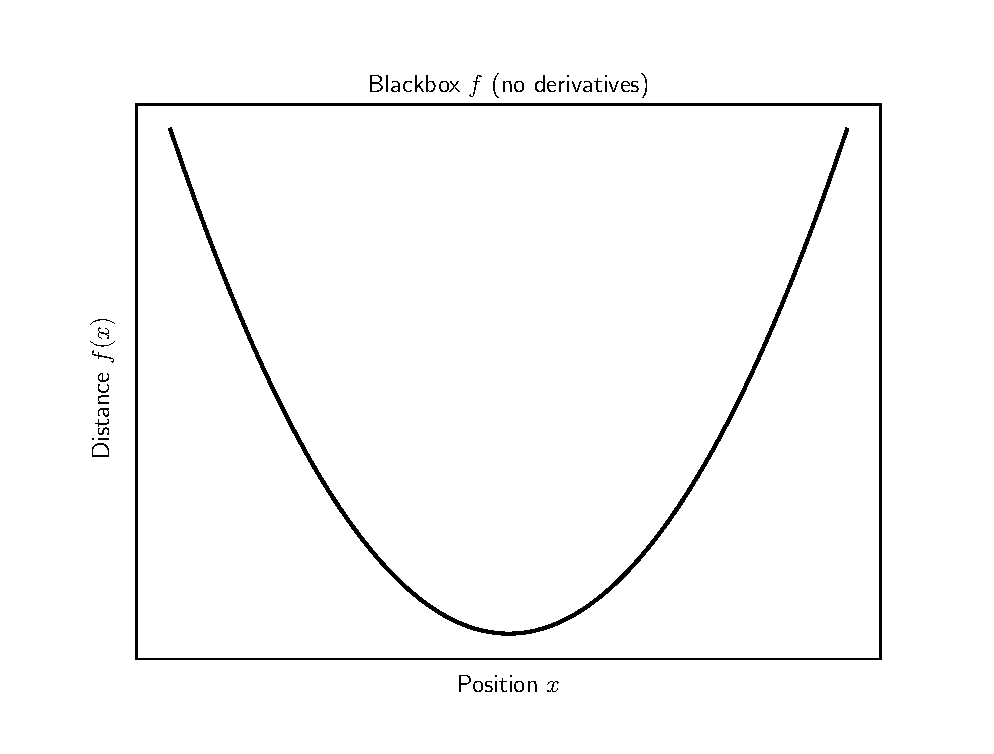
\includegraphics[height=2in]{linear_surrogate_pt1.eps}
}

\vskip -2in

\onslide<2>{
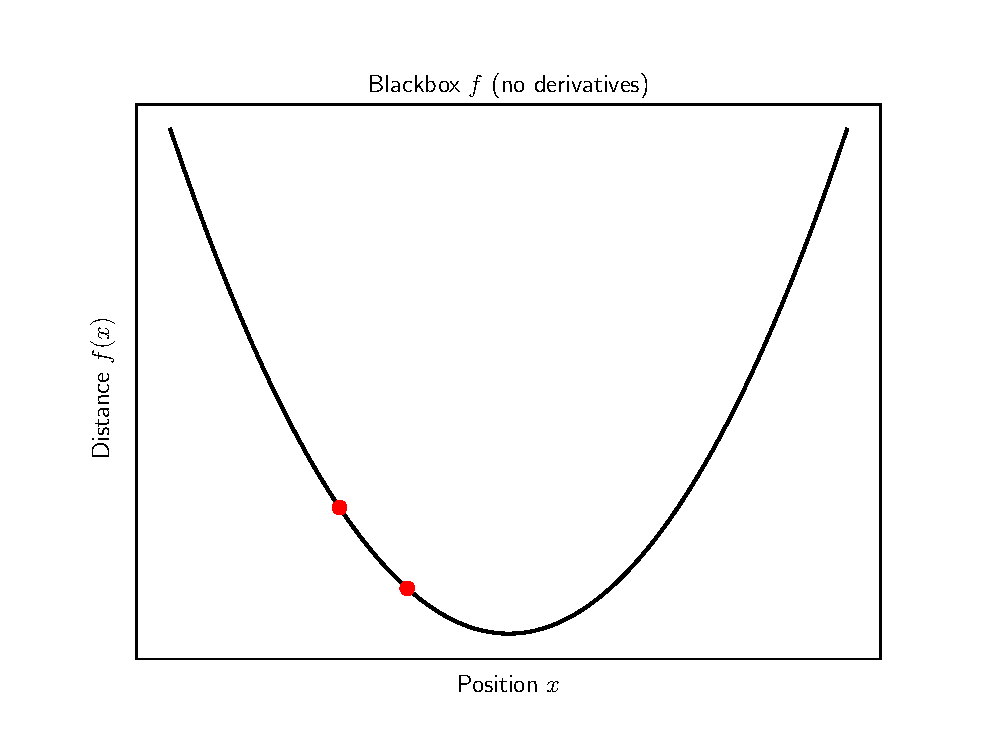
\includegraphics[height=2in]{linear_surrogate_pt2.eps}
}

\vskip -2in

\onslide<3>{
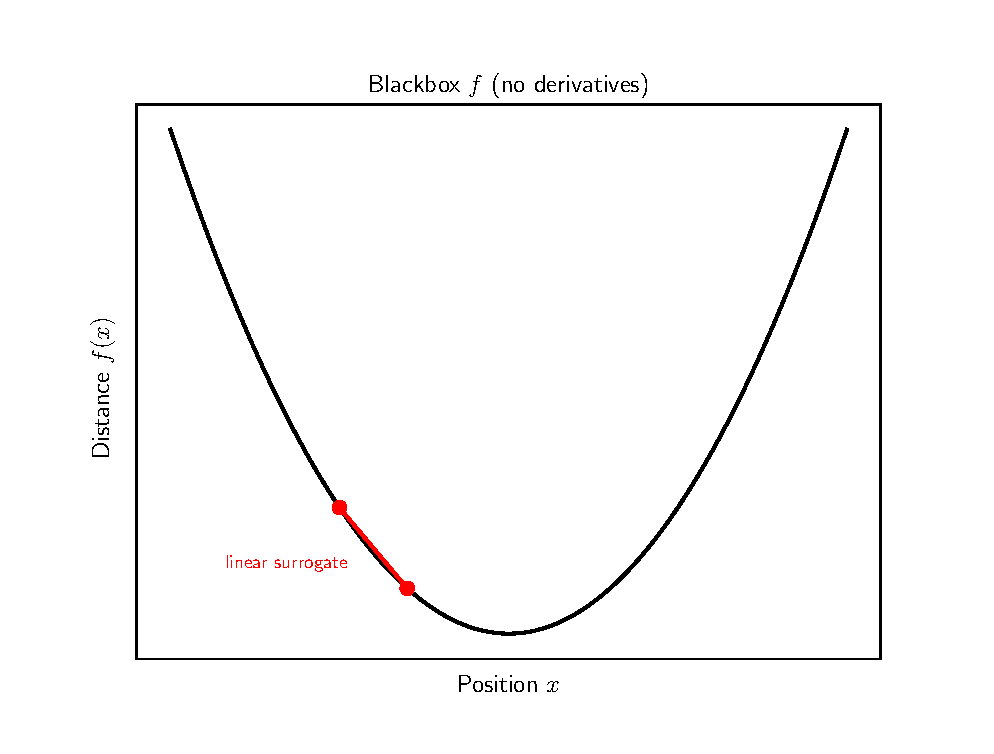
\includegraphics[height=2in]{linear_surrogate_pt3.eps}
}

\vskip -2in

\onslide<4>{
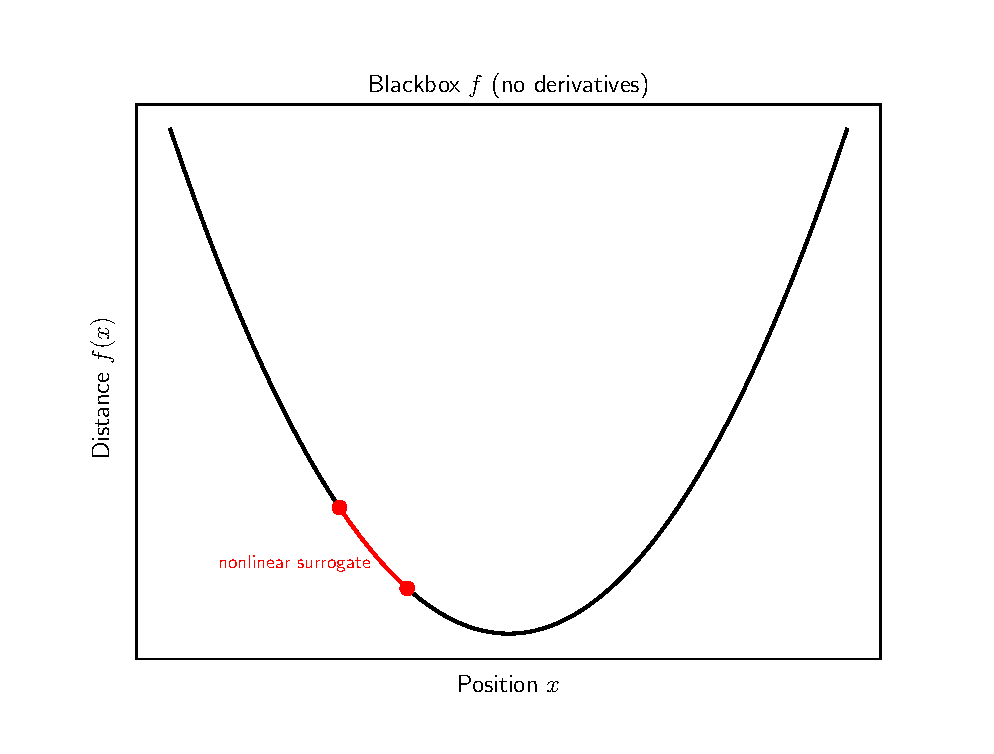
\includegraphics[height=2in]{nonlinear_surrogate_pt3.eps}
}
\end{center}
\end{frame}

\begin{frame}\frametitle{Multiobjective Optimization}
\begin{center}
\onslide<2>{
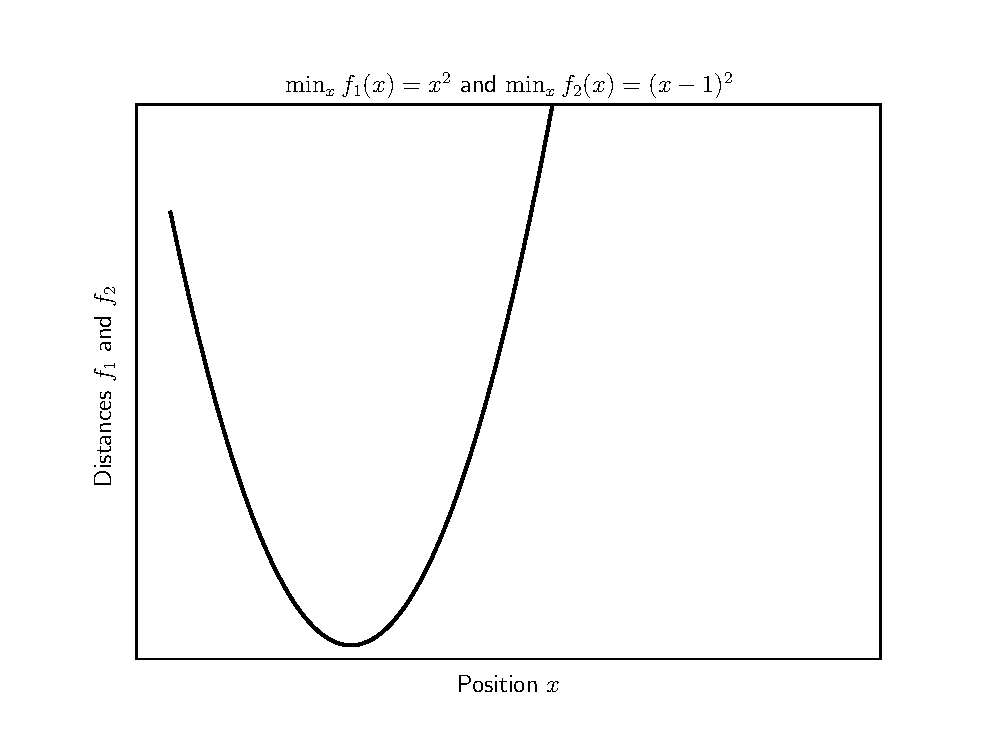
\includegraphics[height=2in]{multi_obj_pt1.eps}
}

\vskip -2in

\onslide<3>{
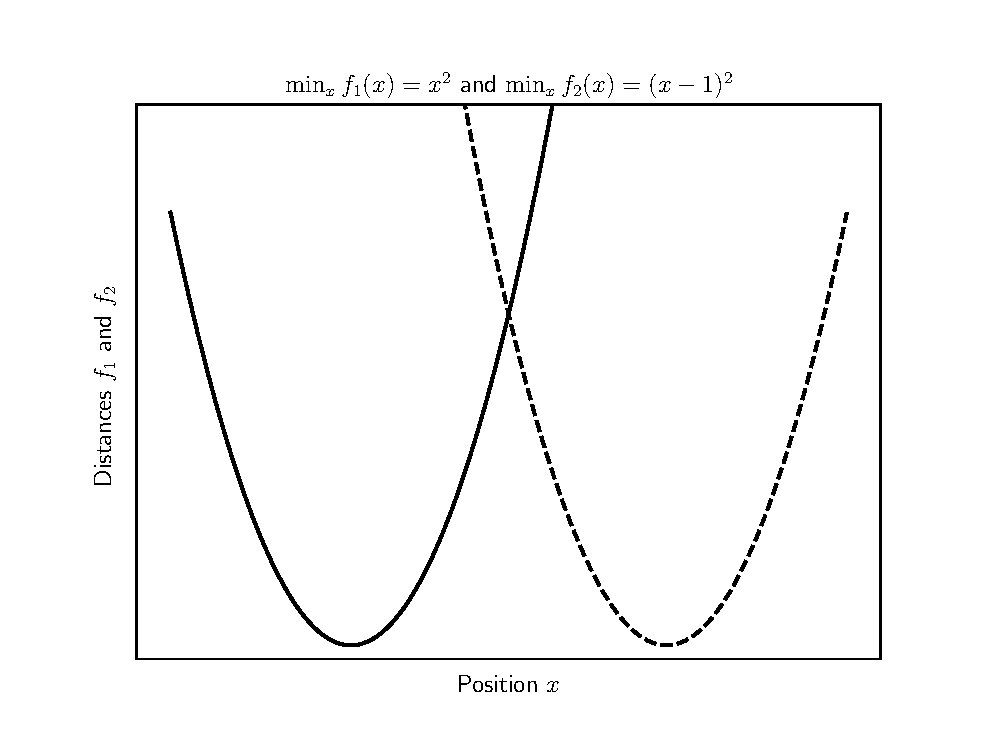
\includegraphics[height=2in]{multi_obj_pt2.eps}
}
\end{center}
\end{frame}

\begin{frame}\frametitle{Dominance Relation}
\begin{center}
\onslide<2>{
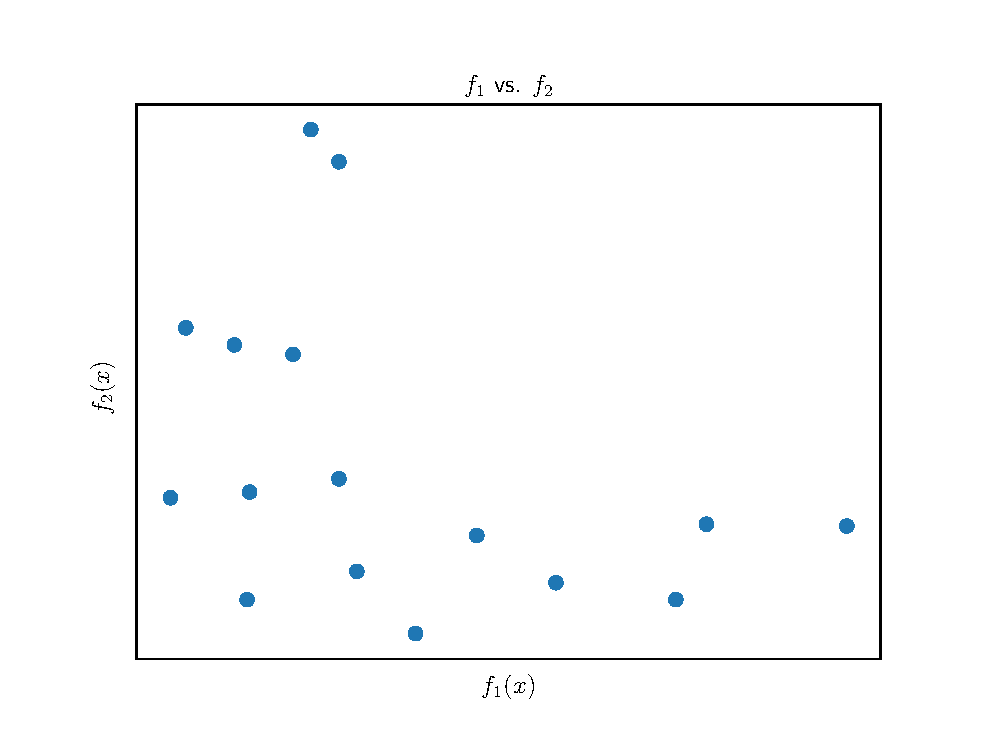
\includegraphics[height=2in]{dominance_pt1.eps}
}

\vskip -2in

\onslide<3>{
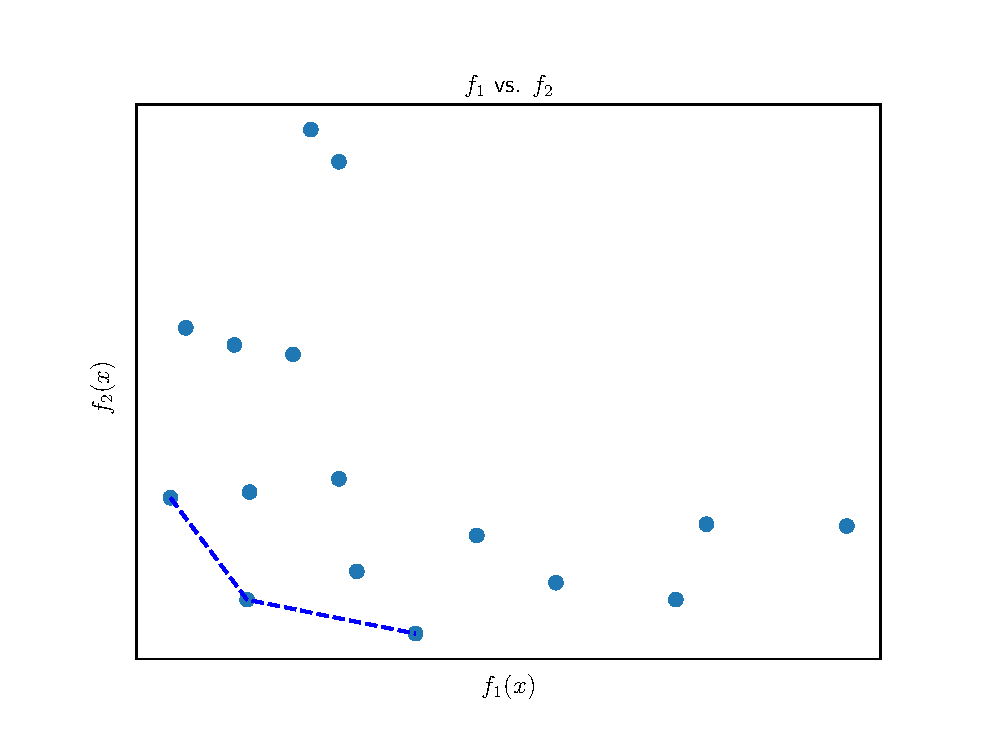
\includegraphics[height=2in]{dominance_pt2.eps}
}
\end{center}
\end{frame}

\begin{frame}\frametitle{Scalarization}
\begin{columns}
\begin{column}{0.5\textwidth}
\onslide<1->{
{\large
$$
\min_{x\in\mathbb{R}^n} \left(f_1(x), f_2(x), \ldots, f_o(x)\right) = F(x)
$$
}}
\onslide<2->{
{\large
$$
G : \mathbb{R}^o \rightarrow \mathbb{R}
$$
}}
\onslide<3->{
{\large
$$
\min_{x\in\mathbb{R}^n} (G \circ F)(x)
$$
}}
\end{column}
\begin{column}{0.5\textwidth}
\begin{center}
\onslide<4>{
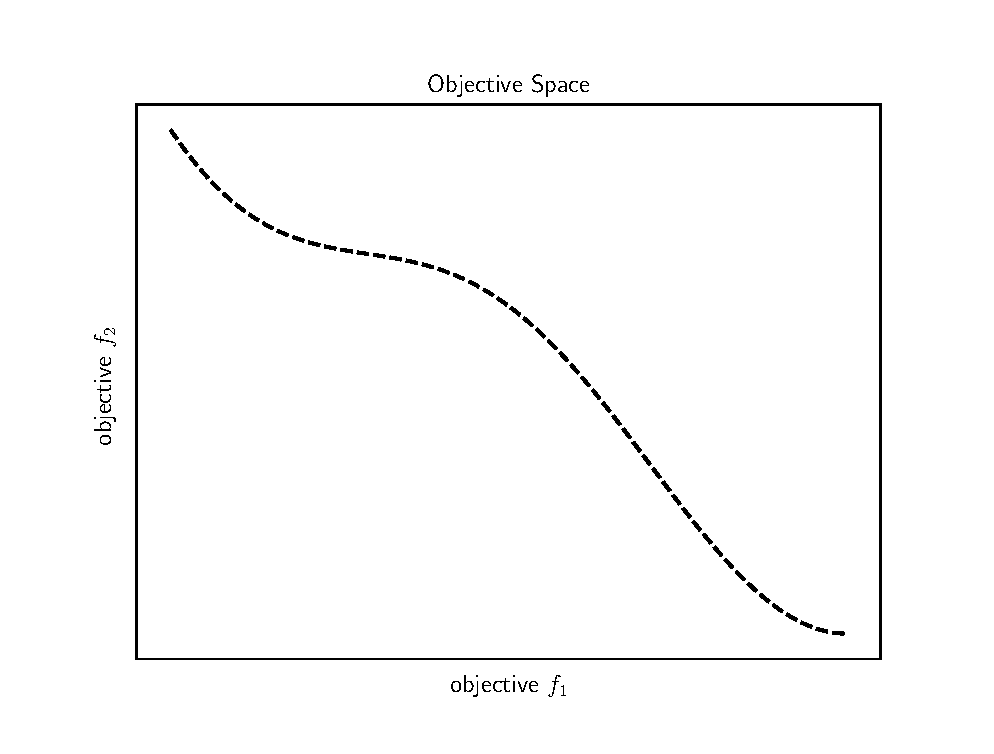
\includegraphics[height=1.5in]{scalarization_pt1.eps}
}

\vskip -1.5in

\onslide<5>{
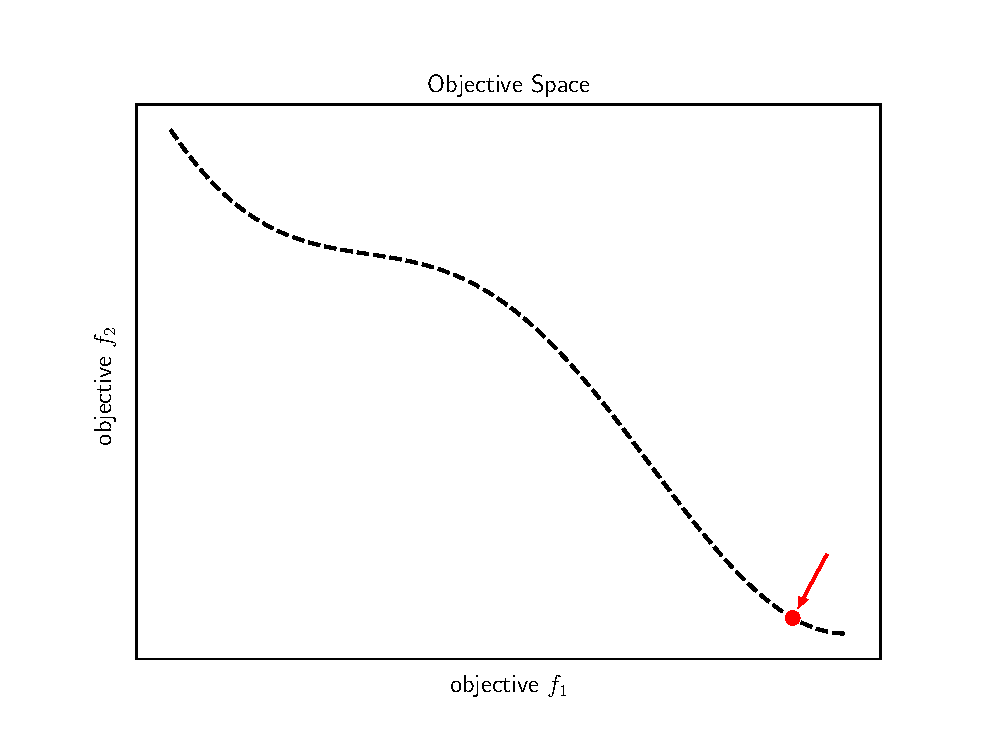
\includegraphics[height=1.5in]{scalarization_pt2.eps}
}

\vskip -1.5in

\onslide<6>{
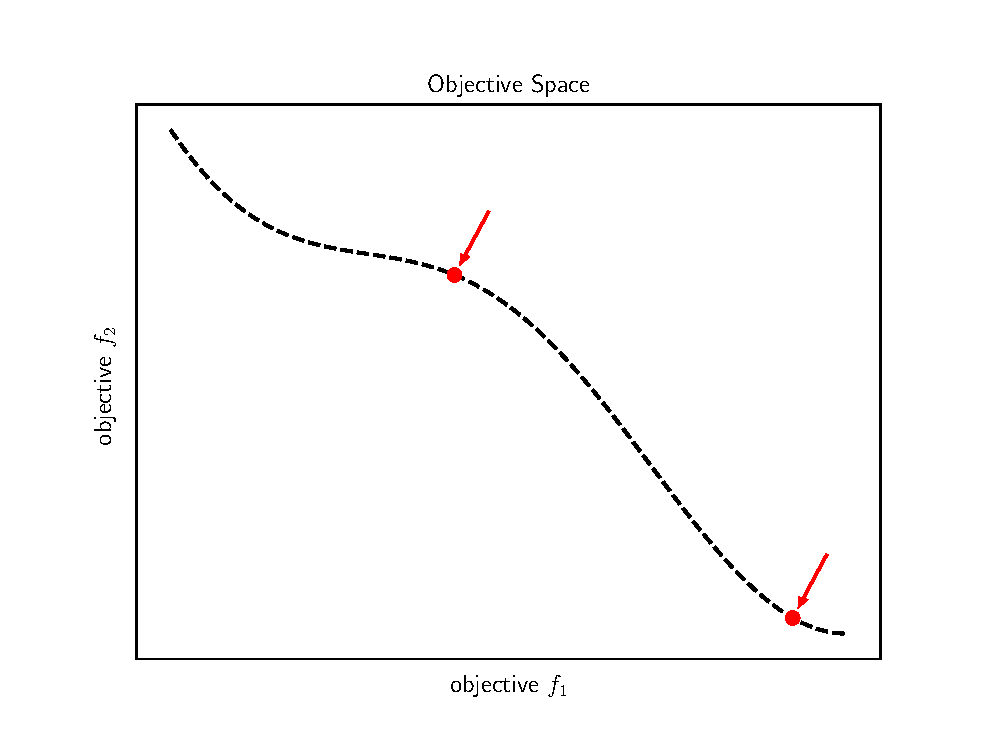
\includegraphics[height=1.5in]{scalarization_pt3.eps}
}

\vskip -1.5in

\onslide<7>{
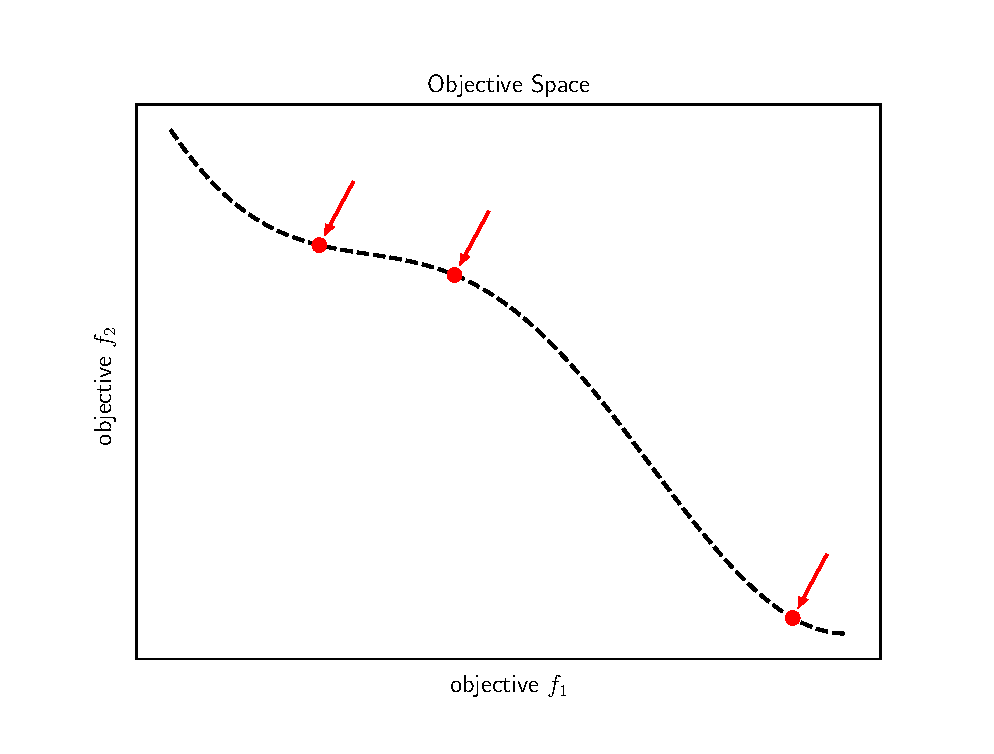
\includegraphics[height=1.5in]{scalarization_pt4.eps}
}
\end{center}
\end{column}
\end{columns}
\end{frame}

\begin{frame}\frametitle{Multiobjective *Simulation* Optimization}
\onslide<1->{
{\bf Problem setting:}\\
\bigskip
\bigskip
\begin{columns}
\begin{column}{.3\textwidth}
Input variables
\end{column}
\begin{column}{.25\textwidth}
\onslide<2>{
Blackbox process}
\end{column}
\begin{column}{.3\textwidth}
Objective space
\end{column}
\end{columns}
\begin{columns}
\begin{column}{.35\textwidth}
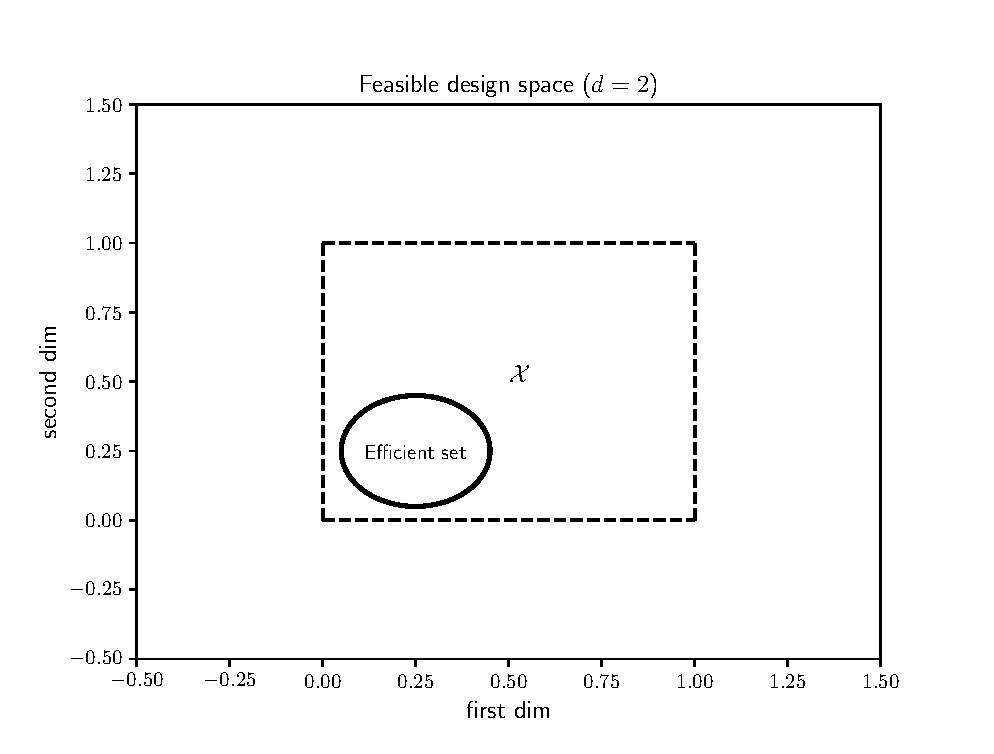
\includegraphics[width=\textwidth]{feasible_design.eps}
\end{column}
\begin{column}{.2\textwidth}
\begin{center}
\onslide<2>{
{\scriptsize
Numerical simulation?\\
Real-world experiment?\\
Build a prototype?\\
Run a test?\\
}}
$\xrightarrow{\hspace*{2cm}}$
$$
F : {\cal X} \rightarrow {\cal Y}
$$
\end{center}
\end{column}
\begin{column}{.35\textwidth}
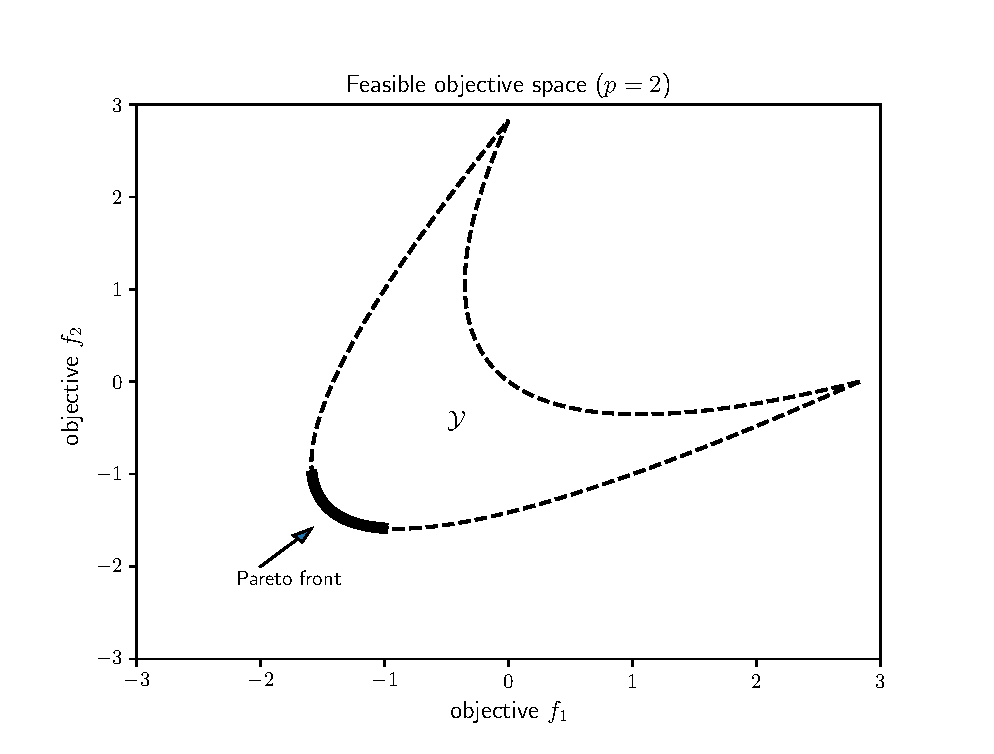
\includegraphics[width=\textwidth]{convex_pareto.eps}
\end{column}
\end{columns}
}
\end{frame}

\begin{frame}\frametitle{ParMOO}
\begin{center}
\onslide<1>{
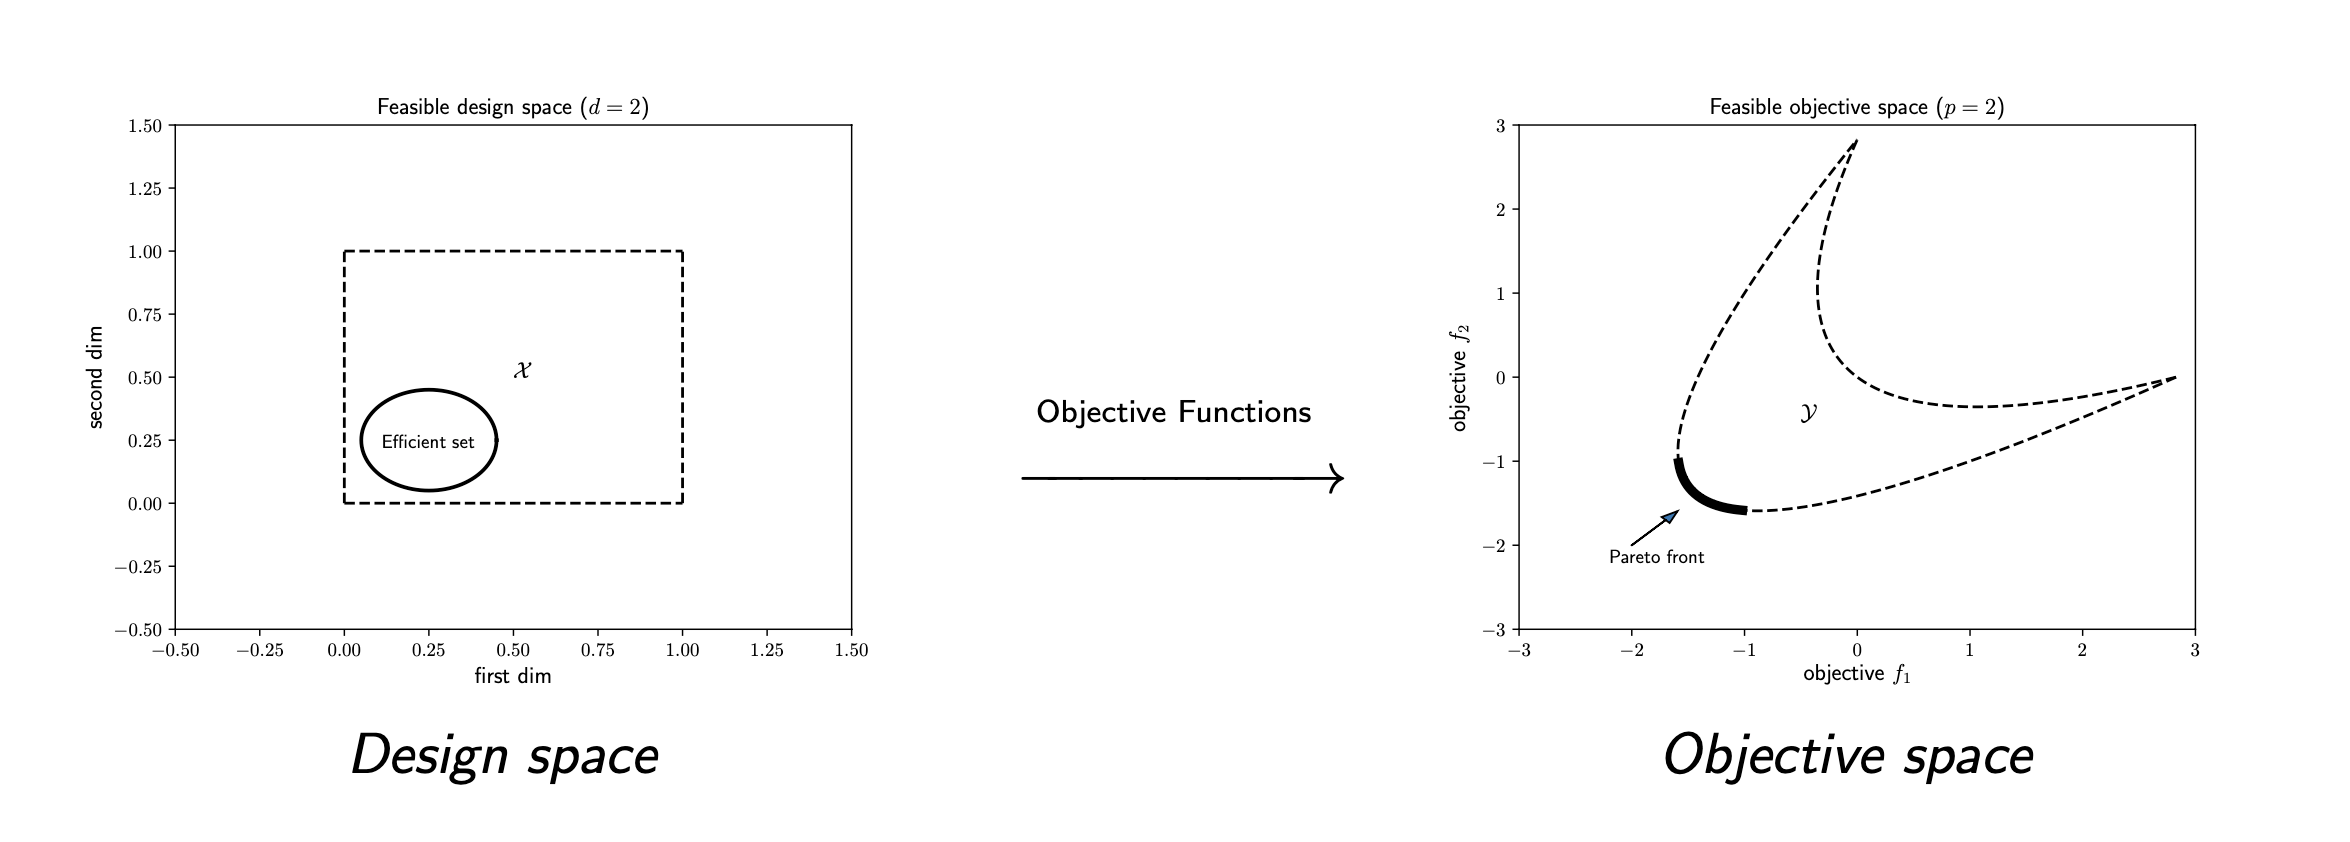
\includegraphics[height=2in]{des-obj-space.png}}

\vskip -2in

\onslide<2>{
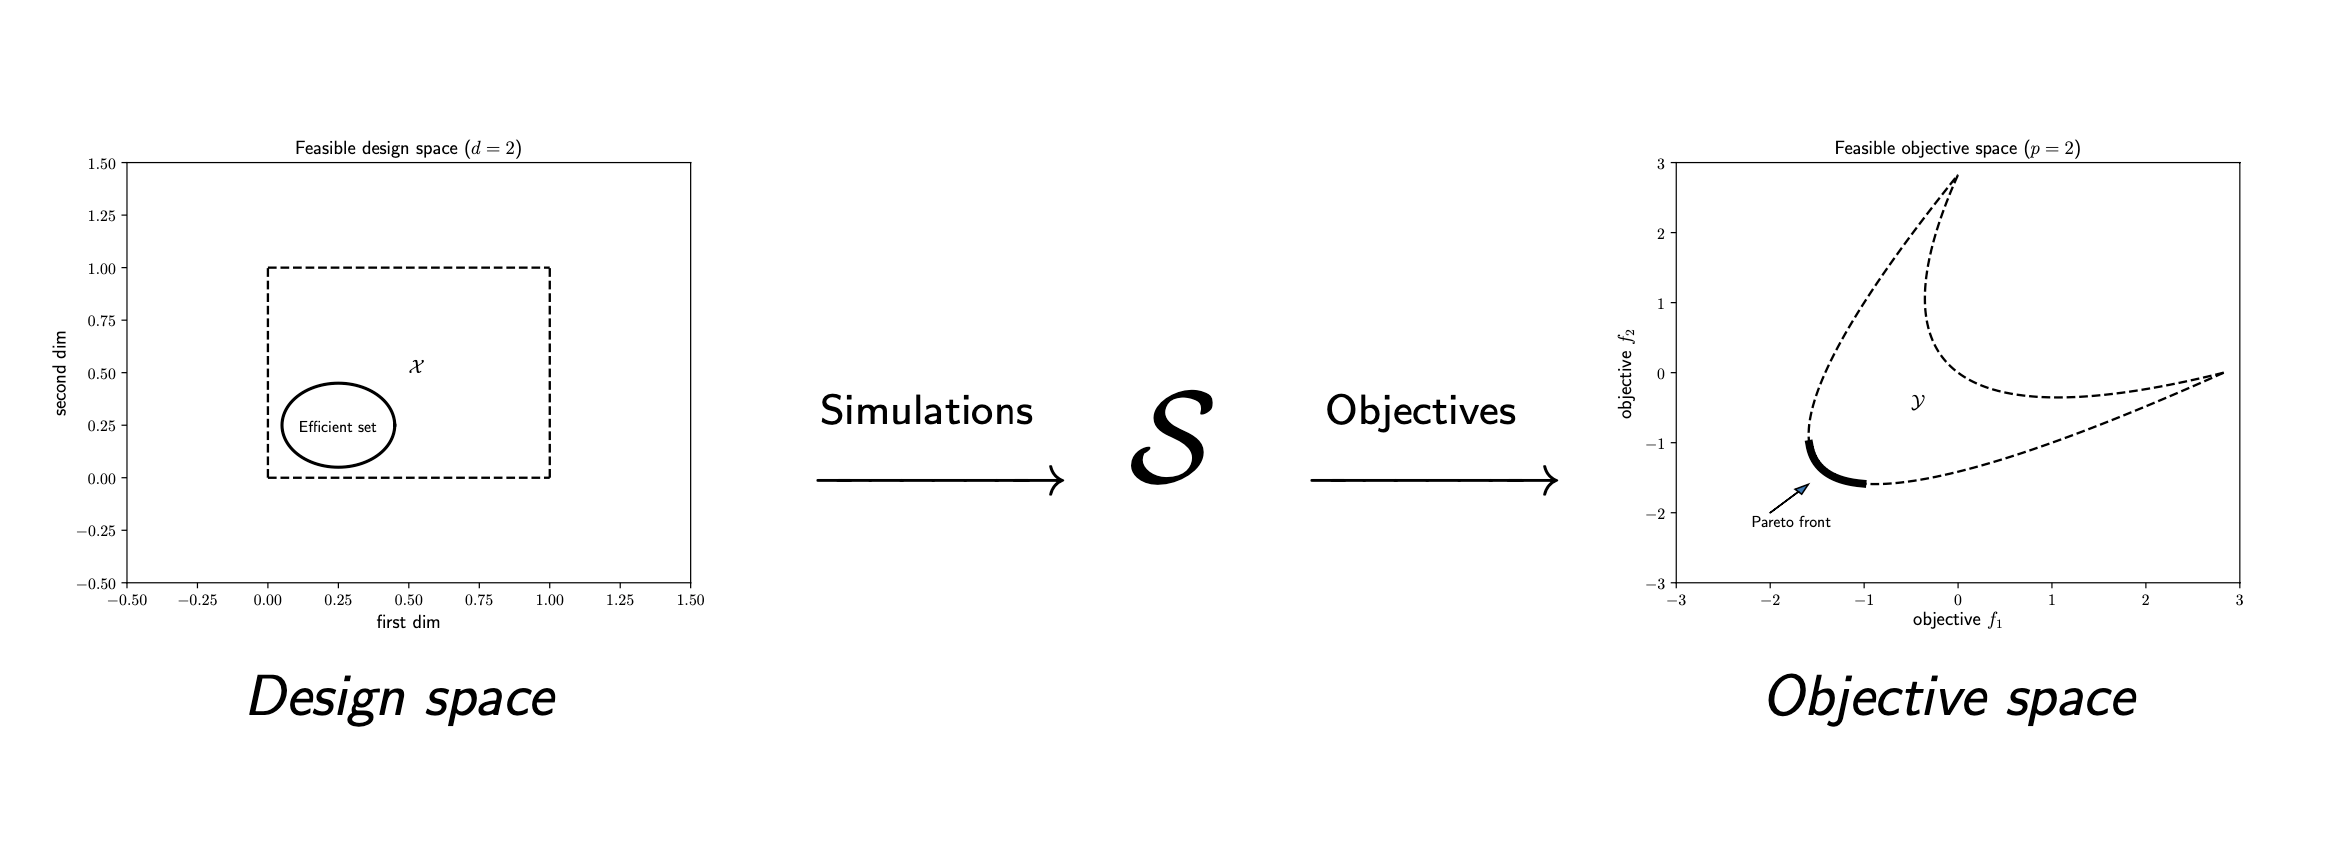
\includegraphics[height=2in]{des-sim-obj-space.png}}
\end{center}
\end{frame}

\begin{frame}\frametitle{ParMOO Solver Components}
\begin{columns}
\begin{column}{0.5\textwidth}

%\includemovie{parmoo.gif}\\
\url{https://parmoo.readthedocs.io/en/latest/quickstart.html}

\end{column}
\begin{column}{0.5\textwidth}
\begin{itemize}
\pause \item Search/DOE technique
\pause \item Surrogate model
\pause \item Acquisition function
\pause \item Single-objective solver
\end{itemize}
\end{column}
\end{columns}
\end{frame}

\begin{frame}\frametitle{ParMOO -- Tutorial}

\begin{center}
{\huge \bf Tutorial}
\end{center}

\end{frame}

\begin{frame}\frametitle{ParMOO -- Other Topics}
\begin{itemize}
\pause \item Constraints
\pause \item Categorical variables
\pause \item Adding derivative option to objectives/constraints
\pause \item Logging and checkpointing
\pause \item Parallel solve using {\tt libEnsemble}
\pause \item Integration with {\tt MDML} (on the {\tt feature/MDML} branch)
\end{itemize}
\end{frame}

\begin{frame}\frametitle{Resources}
\begin{center}
{\large
E-mail: {\tt tchang@anl.gov}\\
E-mail: {\tt parmoo@mcs.anl.gov}\\
\bigskip
\bigskip
ParMOO is under review with JOSS\\
\bigskip
\bigskip
GitHub: {\tt github.com/parmoo/parmoo}\\
Docs: {\tt parmoo.readthedocs.io}\\
PyPI: {\tt pip install parmoo}}

\bigskip
\bigskip

{\small This material is based upon work supported by the U.S. Department of Energy, Office of Science, Office of Advanced Scientific Computing Research, SciDAC program under contract number DE-AC02-06CH11357.}
\end{center}
\end{frame}

\end{document}
